\chapter{Introdução}
  
  Um compilador é um programa que transforma o código de um programa em um outro código, numa linguagem potencialmente diferente da linguagem de entrada\cite{aho:86}. O caso de uso mais comum se dá entre linguagens como \textit{C} e \textit{Fortran} que são traduzidas para o \textit{Assembly}, permitindo expressar instruções de máquina dando como entrada expressões de mais alto nível, ou seja, mais próximas da linguagem natural. Uma outra aplicação recorrente para os compiladores é a otimização de programas. Neste caso, a saída pode estar escrita na mesma linguagem que a entrada, representando o mesmo programa, mas com uma sequência de instruções mais eficiente que o original. \par
  \begin{figure}[H]
    \centering
    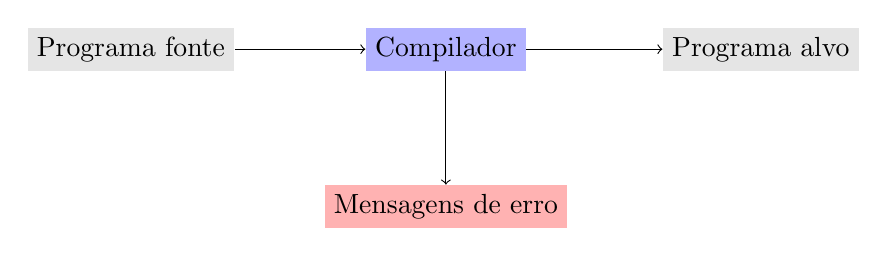
\begin{tikzpicture}[nodes={fill=gray!20},
    row sep=0.3cm,column sep=0.5cm]
        \node[rectangle] (input) at (0,0) {Programa fonte};
        \node[rectangle, fill=blue!30] (compiler) at (4, 0) {Compilador};
        \draw[->] (input) to[out=0,in=180] (compiler);
        \node[rectangle] (target) at (8, 0) {Programa alvo};
        \draw[->] (compiler) to[out=0,in=180] (target);
        \node[rectangle, fill=red!30] (error) at (4, -2) {Mensagens de erro};
        \draw[->] (compiler) to (error);
    \end{tikzpicture}
    \label{fig:compiler-flow}
    \caption{A estrutura básica de um compilador.}
\end{figure}